% !TeX spellcheck = en_GB
% !TeX program = lualatex
%
% v 2.3  Feb 2019   Volker RW Schaa
%		# changes in the collaboration therefore updated file "jacow-collaboration.tex"
%		# all References with DOIs have their period/full stop before the DOI (after pp. or year)
%		# in the author/affiliation block all ZIP codes in square brackets removed as it was not %         understood as optional parameter and ZIP codes had bin put in brackets
%       # References to the current IPAC are changed to "IPAC'19, Melbourne, Australia"
%       # font for ‘url’ style changed to ‘newtxtt’ as it is easier to distinguish "O" and "0"
%
\documentclass[a4paper,
               %boxit,        % check whether paper is inside correct margins
               %titlepage,    % separate title page
               %refpage       % separate references
               %biblatex,     % biblatex is used
               keeplastbox,   % flushend option: not to un-indent last line in References
               %nospread,     % flushend option: do not fill with whitespace to balance columns
               %hyphens,      % allow \url to hyphenate at "-" (hyphens)
               %xetex,        % use XeLaTeX to process the file
               %luatex,       % use LuaLaTeX to process the file
               ]{jacow}
%
% ONLY FOR \footnote in table/tabular
%
\usepackage{pdfpages,multirow,ragged2e} %
\usepackage{tablefootnote}
\usepackage{booktabs}
% CHANGE SEQUENCE OF GRAPHICS EXTENSION TO BE EMBEDDED
% ----------------------------------------------------
% test for XeTeX where the sequence is by default eps-> pdf, jpg, png, pdf, ...
%    and the JACoW template provides JACpic2v3.eps and JACpic2v3.jpg which
%    might generates errors, therefore PNG and JPG first
%
\makeatletter%
	\ifboolexpr{bool{xetex}}
	 {\renewcommand{\Gin@extensions}{.pdf,%
	                    .png,.jpg,.bmp,.pict,.tif,.psd,.mac,.sga,.tga,.gif,%
	                    .eps,.ps,%
	                    }}{}
\makeatother
\newcommand{\ts}{\textsuperscript}
% CHECK FOR XeTeX/LuaTeX BEFORE DEFINING AN INPUT ENCODING
% --------------------------------------------------------
%   utf8  is default for XeTeX/LuaTeX
%   utf8  in LaTeX only realises a small portion of codes
%
\ifboolexpr{bool{xetex} or bool{luatex}} % test for XeTeX/LuaTeX
 {}                                      % input encoding is utf8 by default
 {\usepackage[utf8]{inputenc}}           % switch to utf8

\usepackage[portuguese]{babel}
\usepackage{subcaption}
\usepackage{siunitx}
\usepackage{hyperref}

%
% if BibLaTeX is used
%
\ifboolexpr{bool{jacowbiblatex}}%
 {%
  \addbibresource{jacow-test.bib}
  \addbibresource{biblatex-examples.bib}
 }{}
\listfiles

%%
%%   Lengths for the spaces in the title
%%   \setlength\titleblockstartskip{..}  %before title, default 3pt
%%   \setlength\titleblockmiddleskip{..} %between title + author, default 1em
%%   \setlength\titleblockendskip{..}    %afterauthor, default 1em

\begin{document}

\title{Otimização de Abertura Dinâmica com o RCDS}

\author{Envolvidos: Ana, Fernando, Liu, Matheus, Murilo, Ximenes \\ FAC - LNLS \\ Quarta-feira, 14 de dezembro de 2022}
\maketitle
%
\section{Resumo}
% O \textit{Robust Conjugate Direction Search} (RCDS), um algorítimo de otimização online, foi recentemente integrado aos sistemas de controle de aceleradores (\href{https://github.com/lnls-fac/apsuite/blob/64708a77ebff0c093700b6c5e78a882ed3edd63a/apsuite/optimization/rcds.py}{script}) e testado na otimização da eficiência de injeção mediante variações de \textit{Pos-Ang} na TS e força do NLK (\href{https://github.com/lnls-fac/apsuite/blob/64708a77ebff0c093700b6c5e78a882ed3edd63a/apsuite/commisslib/rcds_posang.py}{classe de medida}). 
Realizamos a otimização online da abertura dinâmica do SIRIUS mediante variações das forças dos sextupolos. Foram adotadas duas funções-objetivo: a taxa de perda de feixe mediante \textit{kicks} dipolares e a eficiência de injeção. Em ambos os casos foi possível otimizar o objetivo. No primeiro deles, entretanto, não obtivemos uma boa eficiência de injeção após a ciclagem. No segundo caso, a otimização resultou em configurações de máquina que renderam eficiências de 95--100\%, com boa repetibilidade, mas com piora do tempo de vida. Verificamos também \textit{drifts} de cromaticidade no decorrer das iterações da otimização de eficiência de injeção.
\section{O algoritmo}
O robust conjugate direction search (RCDS) é um algoritmo de otimização online robusto aos ruídos de medida da função objetivo (detalhes \href{https://www.slac.stanford.edu/pubs/slacpubs/15250/slac-pub-15414.pdf}{aqui}.)
Os \textit{inputs} do algoritmo são a função objetivo (um indicador da abertura dinâmica, neste caso), o nível de ruído experimental da função objetivo, o \textit{range} de variação de cada um dos botões (famílias de sextupolos), o \textit{step} inicial dado na busca do \textit{bracket} (intervalo que contém o mínimo) ao longo de cada direção, as direções iniciais de procura (usamos direções canônicas) e os valores iniciais dos botões (posição inicial no espaço de parâmetro), além dos possíveis critérios de parada: número de avaliações da função objetivo, número de iterações ou tolerância de variação.

\section{Setup do Experimento e Resultados}
Os botões de otimização foram as famílias de sextupolos SDA0, SDB0, SDP0, SFA0, SFB0, SFP0, SDA1, SDB1, SDP1, SDA3, SDB3, SDP3, SFA1, SFB1, SFP1. As famílias SDA2, SDB2, SDP2 e SFA2, SFB2, SFP2 foram usadas para garantir que a ação dos botões de otimização não alterasse a cromaticidade de operação da máquina. Isto foi implementado da seguinte forma: para cada variação proposta pelo algoritmo aos botões de otimização, calculávamos qual seria a variação de cromaticidade e determinávamos a variação de força nas famílias de correção de modo a anular a mudança de cromaticidade \footnote{Usamos a matriz jacobiana de cromaticidade por variações de sextupolos, obtida do modelo}. 
%À máquina eram aplicadas as forças propostas aos botões de otimização, acrescidas das forças de correção, de modo que, em princípio, apenas variações isocromáticas eram aplicadas à máquina.
Testamos a otimização com duas funções objetivo:
\subsection{Otimização da resiliência a kicks}
A primeira função objetivo adotada foi a taxa de perda do feixe após um \textit{kick} dos \textit{pingers} dipolares. A ideia era minimizar a perda para um dado \textit{kick} e ir aumentando os \textit{kicks} a cada rodada, sondando, assim, uma aceitância em ângulo cada vez maior. %A avaliação da função objetivo neste primeiro caso consistia em chutar o feixe e determinar a taxa de perda comparando o sinal soma médio ao longo dos BPMs nas primeiras 10 e com o sinal soma médio nas últimas 10 aquisições de posição.
A taxa de perda era calculada por meio da comparação entre o sinal soma médio das primeiras 10 e as últimas 10 medidas durante a aquisição de BPMs após o \textit{kick} dipolar.

Partindo da ref-config, configuramos o \textit{kick} na horizontal em $\Delta x^\prime = -0.760~ \unit{m rad}$, que rendia uma taxa de perda girando em torno de 35 - 60\% . Um \textit{kick} na vertical $\Delta y^\prime = 0.03~\unit{m rad}$ também era disparado.

\subsubsection{Resultados}
Em uma iteração, a taxa de perda foi de aproximadamente 60\% para 0 (ver Figura~\ref{beam_loss_hist}). A cada avaliação da função objetivo ao longo das 15 direções no espaço de parâmetros observou-se a queda sistemática da função objetivo. Ao iniciar a segunda iteração, verificamos que a função objetivo tomou valores negativos e interrompemos a rodada. As configurações das famílias de sextupolos antes e após a rodada de otimização, bem como suas respectivas variações são apresentadas na Figura~\ref{beam_loss_sexts}. 
\begin{figure}
    \centering
    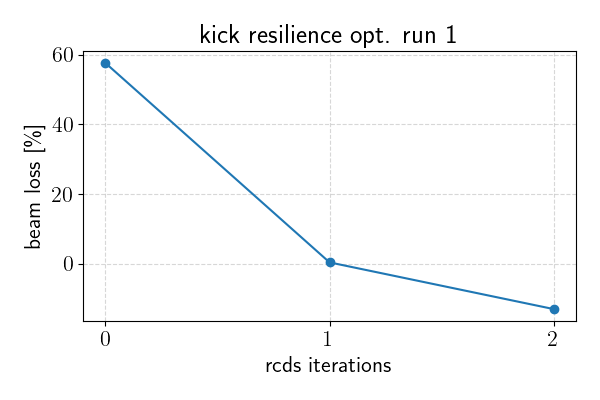
\includegraphics[width=\columnwidth]{beam_loss_hist_run1.png}
    \caption{Histórico da função objetivo ao longo das iterações da primeira rodada de otimização de taxa de perda.}
    \label{beam_loss_hist}
\end{figure}

 O procedimento de minimização da taxa de perda aumentou significativamente a resiliência do feixe. Foi necessário chutá-lo com aproximadamente $0.850~\unit{m rad}$ para obter a taxa de 30--40\% de perda. A máquina foi ciclada e, ao fim do procedimento, verificamos uma eficiência de injeção baixa. A resiliência ao \textit{kick} se manteve, o que levantou  a suspeita de que a abertura em $-x$ tenha sofrido prejuízos com o procedimento de otimização, enquanto a abertura em $x^\prime$ foi maximizada. Partimos então para otimização com outra função objetivo, com esperanças de otimizar simultaneamente as aberturas em posição e em ângulo. 

\begin{figure*}[t]
    \centering
    \includegraphics*[width=\textwidth]{beam_loss_sexts.png}
    \caption{Configurações das famílias de sextupolos ao fim da primeira rodada de otimização de taxa de perda}
    \label{beam_loss_sexts}
\end{figure*}


\subsection{Otimização de eficiência de injeção}
Partindo da configuração de referência, pioramos as condições de injeção reduzindo a intensidade dos \textit{kicks} do NLK de $-2.45~\unit{m rad}$ para $-2.25~\unit{m rad}$. Desse modo o feixe era injetado na beirada esquerda superior da abertura $(x,x^\prime)$, com uma eficiência de injeção em torno de 30 \%. Adotamos como função objetivo o negativo da eficiência de injeção. Sua maximização seria uma consequência do aumento da abertura tanto em posição quanto em ângulo nestas condições de injeção. 
\subsubsection{Resultados}
A primeira rodada de otimização foi disparada e em três iterações do algorítmo atingimos 70\% de eficiência. O algoritmo foi encerrado por ter atingido o máximo número de avaliações da função objetivo (100). Partimos destas configurações e disparamos outra rodada. Em mais quatro iterações atingimos 85\% de eficiência de injeção. Restauramos o NLK ao valor de referência e realizamos a injeção após rápida otimização de pos-ang. A eficiência flutuou em torno de 95--100\% com bastante repetibilidade e houve piora no tempo de vida. 
As configurações e variações das famílias de sextupolos ao fim das rodadas de otimização de eficiência são apresentadas nas Figuras~\ref{inject_sexts1} e~\ref{inject_sexts2}.
\begin{figure}
    \centering
    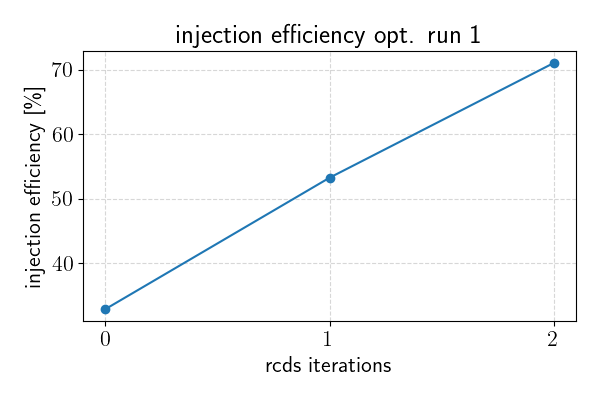
\includegraphics[width=\columnwidth]{injeff_hist_run1.png}
    \caption{Objetivo ao longo das iterações na segunda rodada de otimização de eficiência de injeção}
    \label{injeff_hist1}
\end{figure}

\begin{figure}
    \centering
    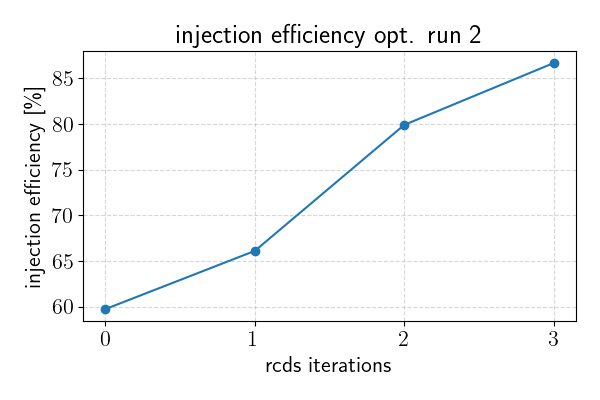
\includegraphics[width=\columnwidth]{injeff_hist_run2.png}
    \caption{Objetivo ao longo das iterações na segunda rodada de otimização de eficiência de injeção}
    \label{injeff_hist2}
\end{figure}


\begin{figure*}[]
    \centering
    \includegraphics*[width=1\textwidth]{sexts_injeff_run1.png}
    \caption{Configurações das famílias de sextupolos ao fim da primeira rodada de otimização de eficiência de injeção}
    \label{inject_sexts1}
\end{figure*}


\begin{figure*}[]
    \centering
    \includegraphics*[width=\textwidth]{sexts_injeff_run2.png}
    \caption{Configurações das famílias de sextupolos ao fim da segunda rodada de otimização de eficiência de injeção}
    \label{inject_sexts2}
\end{figure*}
\section{Medidas de cromaticidade}
Realizamos medidas de cromaticidade da máquina nas configurações de referência e nas configurações encontradas ao fim das iterações 0, 2, e 3 da última rodada de otimização de eficiência de injeção (figura~\ref{injeff_hist2}). A tabela~\ref{chrom} apresenta os resultados das medidas. Verifica-se um \textit{drift} de cromaticidade, mesmo com o procedimento de de variações isocromáticas implementado. 
\begin{table}[h]
\centering
\begin{tabular}{@{}ccc@{}}
\toprule
configuração & $\xi_x$       & $\xi_y$         \\ \midrule
ref-config   & $2.33\pm0.02$ & $2.531\pm0.008$ \\
iteração 0   & $2.59\pm0.02$ & $3.700\pm0.008$   \\
iteração 2   & $2.72\pm0.04$ & $3.704\pm0.008$ \\
iteraçao 3   & $2.76\pm0.05$  & $3.510\pm0.01$   \\ \bottomrule
\end{tabular}
\caption{Medidas de Cromaticidade}
\label{chrom}
\end{table}

Não tivemos tempo de ciclar a máquina e injetar com as configurações ótimas encontradas para verificar se as condições de injeção se manteriam.
% \begin{figure}[h]
%   \centering
%   \includegraphics*[width=1.0\columnwidth]{posang_hist.pdf}
%   \caption{Melhores eficiências vs. iterações p/ cada rodada.}
%   \label{fig:effi}
% \end{figure}

% \begin{figure}[h]
%   \centering
%   \includegraphics*[width=1.0\columnwidth]{after_opt.pdf}
%   \caption{Valor dos botões ao fim das rodadas de otimização}
%   \label{fig:after}
% \end{figure}

\end{document}
